\chapter{Umsetzung}
\section{Datenverarbeitung in CAD}
\label{sec:DatenverarbeitungInCAD}
\subsection{Anwendungsbereiche von CAD}
\label{subsec:AnwendungsbereicheVonCAD}
Die Grundlage dieser Arbeit sowie des Prototypen bilden Daten, welche in 3D-CAD-Programmen erstellt wurden. Daher wird im Rahmen dieser Arbeit CAD als Synonym für 3D-CAD verwendet. Im Gegensatz zu 2D-CAD Systemen können in 3D-CAD Systemen Produkte realer konstruiert werden. Das kann sich positiv auf die Entwicklungszeit auswirken. Kollisionsbetrachtungen ermöglichen eine Fehlererkennung, bevor das erste Teil gefertigt wird.\footnote{Vgl. Dipl. Ing. (FH) Bettina Clauß, Helmut Prof. Dr.-Ing. von Eiff (2013): \textit{CAD Grundkurs}. Hochschule Esslingen, S. 2.} Es ist möglich in CAD anhand von Materialeigenschaften physikalische Eigenschaften wie z.B. Festigkeit, Elastizität etc. zu simulieren. Aufgrund dieser Flexibilität sind CAD-Programme heute in fast allen technischen Zweigen vertreten, darunter Architektur, Bauingenieurwesen, Maschinenbau, Elektrotechnik bis hin zur Zahntechnik.\footnote{Vgl. Wikipedia  (2018): \textit{CAD}.\newline
\url{https://de.wikipedia.org/w/index.php?title=CAD&oldid=178934444},\newline 
abgerufen am 23.08.2018.}


\subsection{3D-Modellierung in CAD}
\label{subsec:3D-ModellierungInCAD}
In einer 3D-Umgebung werden Modelle in dreidimensionaler Form modelliert und persistiert. Ein dreidimensionaler Aufbau ermöglicht das Nachbilden einer realitätsnahen Darstellung, das Rendern aus allen Blickwinkeln und Perspektiven sowie eine bessere räumliche Betrachtung. Das Hauptaugenmerk des Ingenieurs liegt dabei vor allem auf Funktionalitäten wie dem technischen Zeichnen, die Erstellung von Arbeitspläne, Montage- und Bedienungsanleitungen oder der technisch visuellen Darstellung, wie der Kollisionsbetrachtung oder der
Zusammenbau-, Einbau- und Montageuntersuchungen. 
Die in dieser Arbeit thematisierte Betrachtung bezieht sich vor allem auf die Nutzung außerhalb der CAD-Umgebung.  Der Vollständigkeit werden nachfolgend alle rechnerinternen Repräsentationen die in CAD vorliegen betrachtet.

\begin{itemize}
\item \textbf{Kantenmodelle:} Kantenmodelle (auch Drahtgitter oder Wireframe) repräsentieren ein Objekt anhand von Kanten. Diese Darstellung enthält keinerlei Informationen über die Flächen oder das Volumen eines Körpers. Kantenmodelle dienen häufig als Hilfsgeometrie, zu Erzeugung von Flächen oder als Darstellungsart von Volumen- oder Flächenmodellen.

\item \textbf{Flächenmodelle:} Als Flächenmodelle werden \glqq hohle\grqq\ Objekte bezeichnet, deren äußere Form durch Flächen beschrieben wird. Eine intuitive Anpassung der Objekthülle ist mit Hilfe von Kontrollpunkten oder Kontrollnetzen ohne Einschränkung möglich. Unter Zuhilfenahme von analytisch beschreibbarer (Translationsflächen, Regelflächen) sowie analytisch nicht beschreibbarer Flächen (B-spline-, NURBS-Flächen) lassen sich jegliche Formen modellieren.

\item \textbf{Volumenmodelle:} Unter Volumenmodelle versteht man Körper, die neben einer Hülle auch eine Materialdichte besitzen, woraus das System automatisch eine Masse interpretiert. Auf diese Weise bleibt die geometrische Konsistenz bei Manipulation des Objektes erhalten. Aufgrund dieses zusätzlichen Parameters kann ein hoher Grad an Automatisierung sichergestellt werden. Es können Eigenschaften wie Trägheit, Schwerpunkt, Gewicht etc. durch das CAD-System automatisch abgeleitet und als Parameter für Simulationen übergeben werden.  
\end{itemize}

Auf alle beschriebenen Modelle lassen sich räumliche Operationen wie Translation, Rotation und Skallierung anwenden. Zusätzlich existieren für jedes Modell spezielle Werkzeuge um diese zu verformen, zu zerschneiden, zu verdrehen oder anderweitig zu manipulieren.\footnote{Vgl. Wikipedia  (2018): \textit{CAD}.\newline
\url{https://de.wikipedia.org/w/index.php?title=CAD&oldid=178934444},\newline 
abgerufen am 23.08.2018.} 

\subsection{Datei- und Exportformate in CAD}
\label{subsec:Datei-undExportformateInCAD}



\clearpage

\section{Aufbereitung der 3D-CAD Daten}
\label{sec:AufbereitungDer3D-CADDaten}



\subsection{Analyse des CAD-Exports}
\label{subsec:AnalyseDesCAD-Exports}
Bevor das aus CAD exportierte Modell in Unity importiert wird sollte selbiges vorher in einem geeigneten 3D-Programm überprüft werden. Für diesen Zweck wird im Rahmen dieser Arbeit auf Autodesk Maya zurückgegriffen. Maya ist eine professionelle Software für Modellierung, Animation und Rendering von 3D Objekten und Szenen.\footnote{Vgl. Autodesk  (2018): \textit{MAYA}.\newline
\url{https://www.autodesk.de/products/maya/overview},\newline 
abgerufen am 30.08.2018.}
\begin{figure}[H]
	\centering
	\captionsetup{width=1\textwidth}
	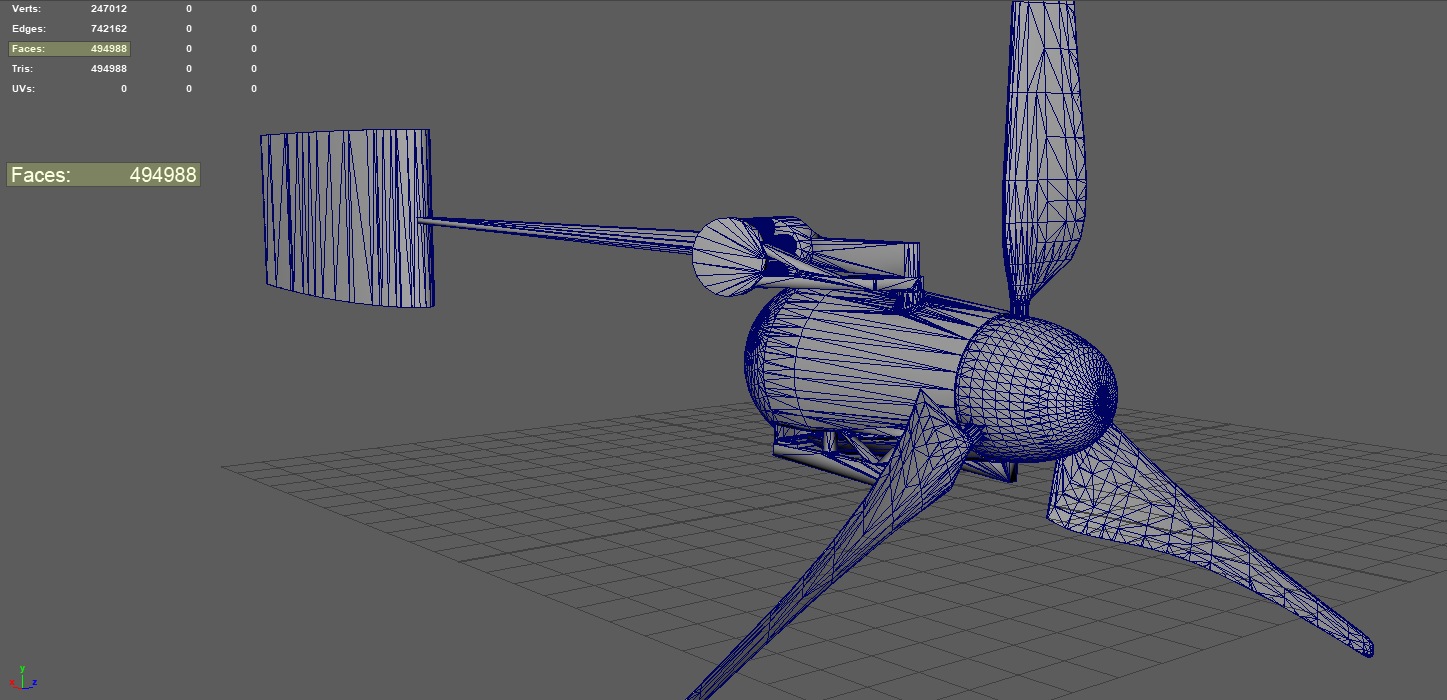
\includegraphics[keepaspectratio, width=1\textwidth]{bildquellen/WEA-Vergleich1}
	\caption{Ergebnis des Exportes der WEA aus der CAD-Anwendung bestehend aus 494.988 Polygonen.}
	\label{fig:2.1}
\end{figure}
Das importierte Modell \sieheAbb{2.1} weist mehrere Eigenschaften auf, welche es für einen Import sowie eine Weiterverarbeitung in Unity ungeeignet machen. Die betreffenden Eigenschaften sind nachfolgend aufgelistet. 
Generell sollten Modelle mit möglichst wenigen Polygonen auskommen, da ein hoher Detailgrad über Texturen generiert werden kann. Im Falle einer technischen Darstellung die neben der äußeren Verkleidung auch innenliegende technische Baugruppen wie Wälzlager, Getriebe o.ä. abbildet, kann dass die Anzahl der Polygone deutlich erhöhen. Schließlich müssen diese in adäquater Qualität dargestellt werden. Natürlich gilt aber auch hier der Grundsatz, dass eine zu geringe Anzahl zu lasten der Darstellungsqualität und eine zu hohe Anzahl zu lasten der Performance geht. Es gilt also einen guten Mittelweg zu finden. 


\begin{itemize}
\item \textbf{Polygon count:} Das Modell besteht aus nicht ganz 500.000 Polygonen, was für eine Echtzeitanwendung sehr viel ist. Laut der Unity Dokumentation sollte der Polycount von dem Zielsystem und der angestrebten Qualität abhängig sein. Das Optimum liegt für Desktopanwendungen bei 1500 bis 4000 Polygonen pro Objekt. Falls sehr viele Objekte zur selben Zeit aktiv sind wird eine Reduktion der Polygone empfohlen.\footnote{Vgl. Unity Documentation  (2018): \textit{Modeling characters for optimal performance}.\newline
\url{https://docs.unity3d.com/Manual/ModelingOptimizedCharacters.html},\newline 
abgerufen am 30.08.2018.}     

\item \textbf{Unterteilung in Einzelobjekte:} Die WEA setzt sich aus vielen Einzelobjekten zusammen. Diese sind vom großen Rotorblatt bis zur kleinsten Schraube zu einem einzigen Objekt zusammengefasst. Es ist also nicht möglich einzelne Teilobjekte in Unity separat mit Materialien und Skripten auszustatten oder zu Animieren.  

\item \textbf{Flächenverteilung:} Ferner führt die ungleichmäßige Flächenverteilung im STL Export zu Darstellungsfehlern beim Shading \sieheAbb{2.2}.
\end{itemize}

\begin{figure}[H]
	\centering
	\captionsetup{width=1\textwidth}
	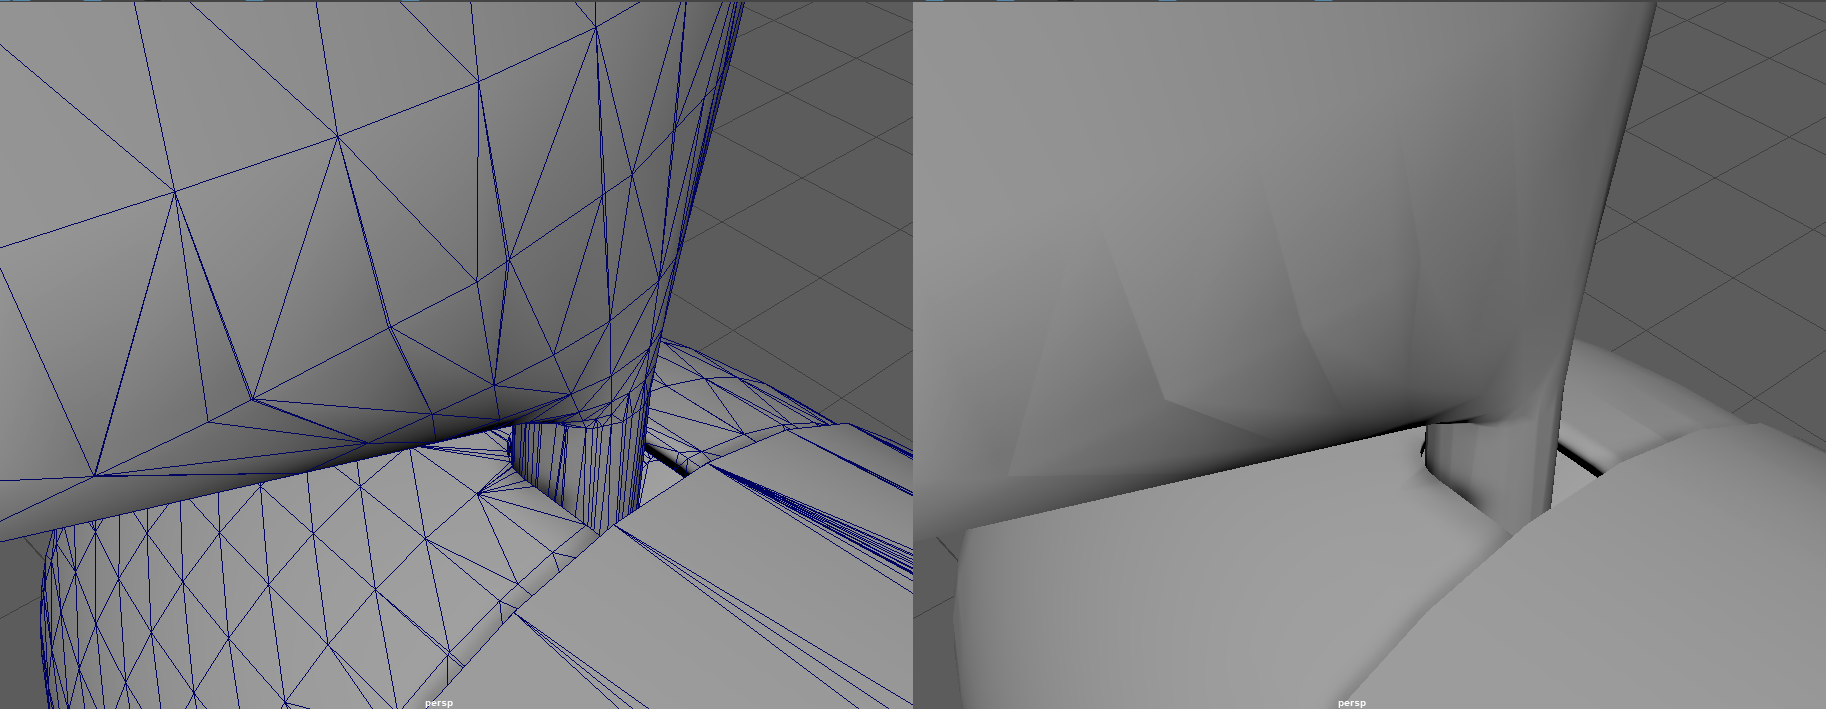
\includegraphics[keepaspectratio, width=1\textwidth]{bildquellen/WEAfehlerhaftesshading}
	\caption{Shadingfehler am Exportmodell.}
	\label{fig:2.2}
\end{figure}

Um diese Probleme zu lösen ist eine Retopologisierung also eine Überarbeitung der Geometrischen Grundstruktur und eine damit einhergehende Reduktion der Flächen nötig.

\begin{figure}[H]
	\centering
	\captionsetup{width=1\textwidth}
	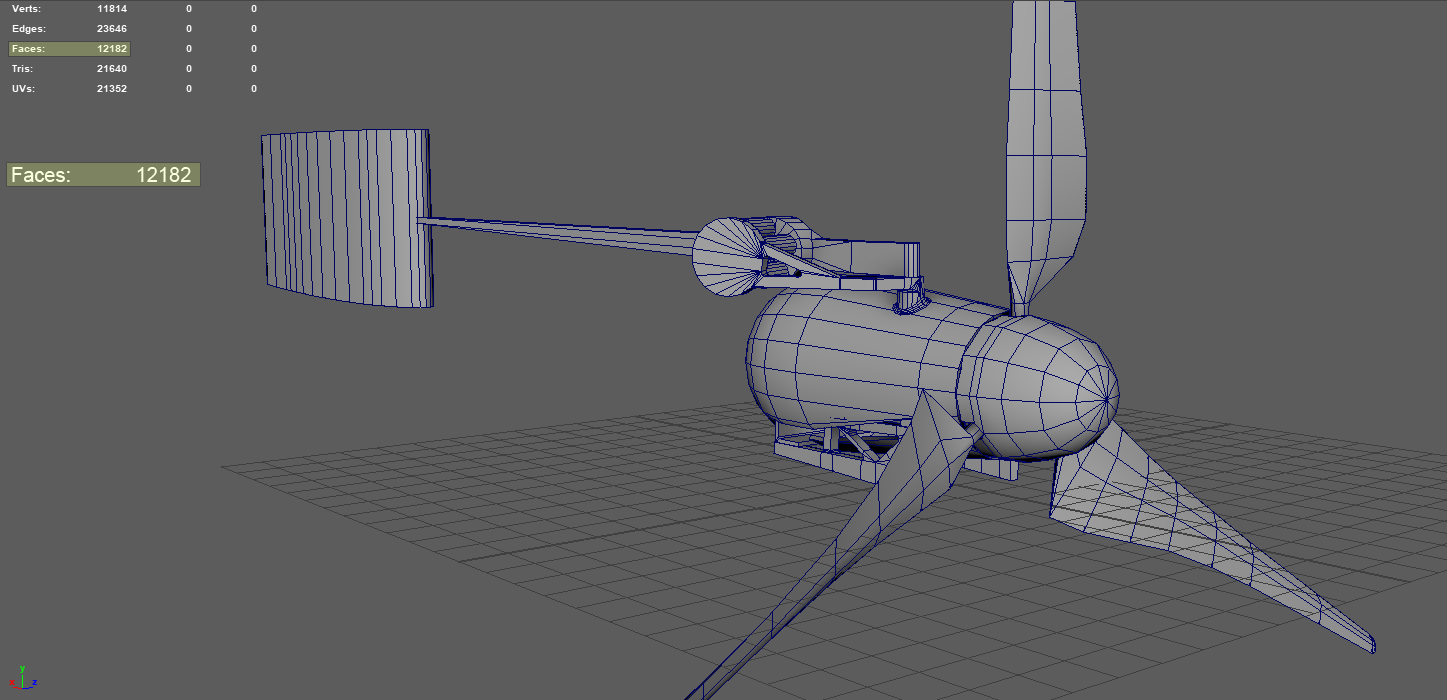
\includegraphics[keepaspectratio, width=1\textwidth]{bildquellen/WEA-Vergleich2}
	\caption{Ergebnis der Retopologisierung bestehend aus 12.182 Polygonen.}
	\label{fig:2.3}
\end{figure}